% Primarily this section should be about scientific methods and theories you need to evaluate/compare/invent to solve your problems from 1.3.
% In some cases it may be ok to describe different technologies, but the purpose is to describe something and then draw a conclusion from that.
% Example, if you decide to discuss different databases, it may be for the purpose of selecting the best type for your implementation later on (based on for example data representation, scalability, speed, etc.).
% Optimally the problems in 1.3 are not solved by anyone else yet, in which case this section needs to describe how to solve them (new algorithms, mathematical approaches, etc.).
 
% This section can have a lot of subsections (3.1, 3.2, 3.3, etc).

% TODO: Explain Evaluation of values

The process of evaluating the value of a variable is a bit complicated because there is a lot of variation.
Thus to simplify the explanation a simple example will be used to explain the main part of evaluating a variable.


Taking a look at the example in figure \ref{fig:subprogramexample} there is a function/subprogram \gls{die} with the name \emph{my\_function}(it is the \gls{die} with the tag \emph{DW\_TAG\_subprogram}).
The function has a parameter called \emph{val} which is the \gls{die} with the tag \emph{DW\_TAG\_formal\_parameter}, it is a child of the function \gls{die}.
Which means that it is a parameter to the function \emph{my\_function}.
It is this parameter \emph{val} that will be used as an example of how to evaluating a variable.


\begin{figure}[h]
	\centering
	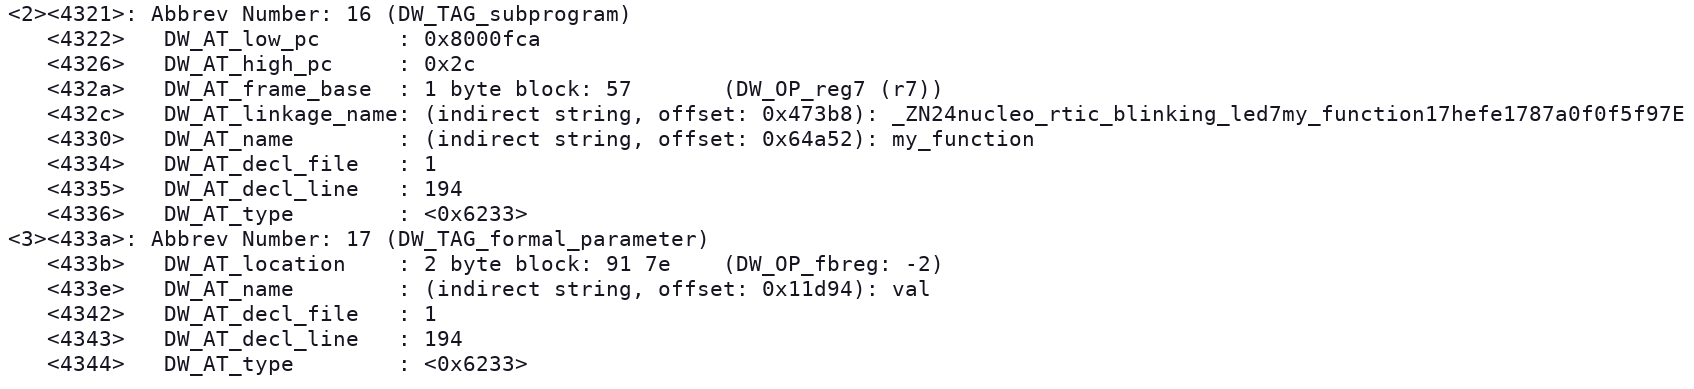
\includegraphics[width=1.0\textwidth]{subprogram-example.png}
	\caption{An example of a subprogram and parameter \gls{DWARF} \gls{die}. This example is the output of the program \emph{objdump} run on a \gls{DWARF} file.}
	\label{fig:subprogramexample}
\end{figure}


A key thing to note is that the function \gls{die} called \emph{my\_function} has two attribute called \emph{DW\_AT\_low\_pc} and \emph{DW\_AT\_high\_pc}.
Those attributes describe the range of \gls{pc} values in which the function is executing.
There is also some other attributes in the example that will not be mentioned because they are not needed for determining the value of the attribute.


%Another important thing to note is that the example explained is a very simple one meaning that there is a lot more different \gls{DWARF} operation for finding the location of a variable and also a lot more different tags for the type \glspl{die}.
%All the various tags for type \glspl{die} requires a unique explanation to how it should be used thus the explanation of each one of them can be read about in the \gls{DWARF} specification \cite{dwarf}, the same goes for the different \gls{DWARF} operations.


\subsubsubsection{Finding Raw Value Location}
Examining the \gls{die} for the argument \emph{val} there is an attribute there called \emph{DW\_AT\_location}.
The value of that attribute is a number of operations, performing these operations will give the location of the variable.


In this example the operation in the \emph{DW\_AT\_location} attribute in figure \ref{fig:subprogramexample} is \emph{DW\_OP\_fbreg $-2$}.
That operation describes that the value is stored in memory at the \emph{frame base} minus $2$(see \cite{dwarf} page 18).
The \emph{Frame base} is the address to the first variable in the functions stack frame(see \cite{dwarf} page 56).


Currently the value of the \emph{frame base} is unknown, but the location of the \emph{frame base}  is described in the \emph{my\_function} \gls{die}.
The location of the \emph{frame base} is also described in a number of operations.
Those operations can be found under the attribute \emph{DW\_AT\_frame\_base}.
Looking at figure \ref{fig:subprogramexample} the \emph{frame base} location is described with the operation \emph{DW\_OP\_reg7}.
The operation \emph{DW\_OP\_reg7} describe that the value is located in register $7$(see \cite{dwarf} page 27).
Thus register $7$ needs to be read to get the value of the \emph{frame base}.


Now knowing the value of the \emph{frame base} the location of the parameter val can be calculated.
As mention the location of parameter \emph{val} is the \emph{frame base} minus $2$.
Thus the value of \emph{val} can be read from the memory at address of the \emph{frame base} minus $2$.
But the value also has to be parsed into the type of \emph{val}, see section \ref{sec:parsingvalue} for how that is done.


\subsubsubsection{Parsing the Raw Value} \label{sec:parsingvalue}
Now the fist problem with parsing the value of the parameter \emph{val} into the correct type is knowing what type the parameter has, this is where the attribute \emph{DW\_AT\_type} comes in.
The value of the \emph{DW\_AT\_type} attribute points to a type \gls{die} tree, which describes the type of the \gls{die}.


The offset to the type \gls{die} of the parameter \emph{val} is $0x6233$, as can be seen in figure \ref{fig:subprogramexample}.
Finding that type \gls{die} is done by going to that offset in the \emph{.debug\_types} section.
The type \gls{die} for \emph{val} can be seen in figure \ref{fig:basetypeexample}, note that the offset of the \glspl{die} tag is the same as $6233$.
That type \gls{die} has the tag \emph{DW\_TAG\_base\_type} which means that it a standard type that is built into most the languages(see \cite{dwarf} page 75).


\begin{figure}[h]
	\centering
	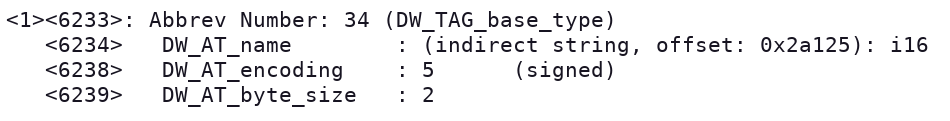
\includegraphics[width=1.0\textwidth]{basetype-example.png}
	\caption{An example of a base type \gls{DWARF} \gls{die}. This example is the output of the program \emph{objdump} run on a \gls{DWARF} file.}
	\label{fig:basetypeexample}
\end{figure}


In this example the type \gls{die} has three attributes which are used to describe the type.
The first attribute is \emph{DW\_AT\_name}, it describes the name of the type.
In this case the name of the type is \emph{i16}, which can be seen in figure \ref{fig:basetypeexample}.
The next attribute is \emph{DW\_AT\_encoding}, this attribute describes the encoding of the type.
An encoding with the value $5$ means that the type is a signed integer\cite{dwarf}.
The different values for encodings are specified in the \gls{DWARF} specification \cite{dwarf}.
Now the last attribute is \emph{DW\_AT\_byte\_size}, it describes the size of the type in bytes.
A byte size of $2$ in this case means that the type is a $16$ bit signed integer.
Now that the type of \emph{val} is known the only thing left to do is to parse the bytes of the value into a signed $16$ bit integer.


